\documentclass[11pt, a4paper, twoside, onecolumn, final]{memoir}

% ------------------------------------------------------------------------
% Margins
\setlrmarginsandblock{35mm}{30mm}{*}
\setulmarginsandblock{40mm}{*}{*}
\OnehalfSpacing
\checkandfixthelayout

% ------------------------------------------------------------------------
% Fonts
\usepackage{fourier}
\usepackage[T1]{fontenc}

% ------------------------------------------------------------------------
% Packages
\usepackage{graphicx}
\usepackage{color}
\usepackage{natbib}	% flexibility of citation format to allow for Harvard
\usepackage{titlesec}
\usepackage{natbib}
\usepackage{lipsum}  % Dummy text generator

% ------------------------------------------------------------------------
% Running footer
\makeevenfoot{plain}{\thepage}{}{}
\makeoddfoot{plain}{}{}{\thepage}

% ------------------------------------------------------------------------
% Document Division
\maxsecnumdepth{subsection}
\maxtocdepth{subsection}

% ------------------------------------------------------------------------
% Define custom chapter style:
\usepackage{anyfontsize}
\newcommand\YUGE{\fontsize{48}{60}\selectfont}

\makechapterstyle{customchap}{%
\setlength{\beforechapskip}{0pt}
\renewcommand*{\chapnumfont}{\YUGE\rmfamily\raggedleft}
\renewcommand*{\chaptitlefont}{\huge\rmfamily\bfseries\raggedleft}
\renewcommand*{\printchapternonum}{%
\vphantom{\printchaptername}%
\vphantom{\chapnumfont 1}%
\afterchapternum
\vskip -\onelineskip}
\renewcommand*{\printchaptertitle}[1]{\chaptitlefont ##1}
\renewcommand*{\printchaptername}{}
\renewcommand*{\printchapternum}{\chapnumfont\thechapter}
}
% ------------------------------------------------------------------------


% ------------------------------------------------------------------------
% MAIN DOCUMENT
\begin{document}

\openleft
	
% Front Matter %	
\frontmatter

% ------------------------------------------------------------------------
% Title Page
  
  {
  \thispagestyle{empty}
	\centering
	\vspace*{0.08\textheight}
	{\Huge\bfseries Title of Thesis}\\[\baselineskip]
	{\Large\scshape Thesis Subtitle}\\[\baselineskip]
	\vfill
	{\large\scshape Full Name}\par
	\vfill
		{\centering
\includegraphics[width = 50mm]{images/rgu_logo.png}} \par
	The Robert Gordon University \par
	School of Health/Computing/Business
	\vfill
	Submitted in partial fulfilment of the requirements of the degree of \par
	Doctor of Philosophy \par
	\vfill
	{\scshape Month, Year}\par
	\vfill
  }
  
% ------------------------------------------------------------------------
	
  \pagestyle{plain}
  
  \cleardoublepage
  
	% Abstract
		\begin{abstract}
	
	\addcontentsline{toc}{chapter}{Abstract}
	
	Metus in vitae nec duis in eu quam mattis in aliquam pede urna purus semper wisi eu commodo ac id aliquet nostrum enim quis neque quis congue neque vestibulum perspiciatis ultrices porta luctus class est libero eros nibh neque vehicula neque nec dui praesent quam risus egestas velit aliquet in urna voluptatibus purus sem quam vestibulum in mauris ut augue in suspendisse fusce purus tempus lacus facilisis magna porro eget fringilla lobortis dignissim tellus quis felis mauris nunc a turpis a lacinia fermentum arcu lectus metus lobortis eu consequuntur eget leo libero pellentesque libero ut litora integer elit sodales adipiscing vitae maecenas quam vestibulum turpis eget suspendisse mattis non sed lacinia diam tristique turpis nullam duis turpis imperdiet tortor in turpis egestas magna interdum sed in ultricies lectus arcu cursus dis vivamus vel aptent faucibus neque ut curabitur vel non velit libero ornare cras wisi convallis sagittis suspendisse eget erat metus vel sollicitudin dui voluptatem in vel lobortis commodo sapien volutpat tortor lectus aenean elementum integer ac rhoncus suscipit ultricies in rutrum ac blandit penatibus integer maecenas aenean curabitur adipiscing gravida phasellus viverra enim viverra sunt ultrices eros assumenda hendrerit wisi commodo arcu dui sodales diam arcu quam vestibulum nonummy ultricies etiam nostra nonummy a enim praesent enim nulla dapibus adipiscing nisl turpis varius consequatur tempor nec tempor adipisicing neque enim sit integer nonummy aliquet felis nulla dui nullam elementum mattis commodo lectus gravida cras morbi tristique aliquam felis rutrum non turpis aliquet imperdiet tellus tellus phasellus diam in vitae luctus magnis gravida wisi in in volutpat tempus suspendisse rutrum dictum impedit torquent sit adipiscing sollicitudin ornare nonummy et pellentesque sapien sociis suscipit turpis egestas magna justo wisi nibh accumsan eget tincidunt dolorum vitae maecenas diam sollicitudin quis dignissim quisque erat amet nec dolor nec sit proin feugiat lectus cras.
	
\end{abstract}
    
    \openright
		
	% Thesis Dedication
		\begin{center}
			\vspace*{7.5cm}
			This thesis is dedicated to my cat / flatmate / parents.
			\addcontentsline{toc}{chapter}{Dedication}
			%\let\cleartorecto\oldcleartorecto % <--- new; restores original macro
		\end{center}
	
	% Acknowledgements %
	% Put the logos of research partners at the bottom of the page %
		\chapter{Acknowledgements}

Include your acknowledgements to Parents, Supervisors,, Friends, Research Partners etc.

\vfill
\begin{center}
	
\includegraphics[scale=0.9]{images/rgu_logo2.jpg}
\end{center}

		\cleardoublepage
	
	% Table of Contents
		\vspace*{-2.5cm}
		\tableofcontents
		\clearpage
	
	% Publictions and Conference Proceedings %
	% A list of published articles and conference proceedings %
	
	% List of Tables %
		\vspace*{-2.5cm}
		\listoftables
		\clearpage
	
	% List of Figures %
		\vspace*{-2.5cm}
		\listoffigures
		\clearpage
	
\chapter{Abbreviations}

\addcontentsline{lot}{table}{Abbreviations}
\begin{table}[th!]
    \centering
		\begin{tabular}{p{1cm}p{11cm}l}
      DNA & Deoxyribonucleic acid & p. 11 \\
      L & \lipsum[2] & p. 11 \\
		\end{tabular}
\end{table}


\chapter{Nomenclature}

\section*{General fluid mechanics}

\addcontentsline{lot}{table}{Nomenclature}
\begin{table}[th!]
    \centering
		\begin{tabular}{p{1cm}p{11cm}l}
      $g$ & Gravitational constant & p. 11 \\
      $L$ & \lipsum[2] & p. 11 \\
		\end{tabular}
\end{table}

\chapter{Glossary}

\addcontentsline{lot}{table}{Glossary}
\begin{table}[th!]
    \centering
		\begin{tabular}{p{2cm}p{11cm}}
      \textbf{Aboriginals} & \lipsum[2] \\
		\end{tabular}
\end{table}

\chapter{Preface}

\lipsum[2-3]

\begin{flushright}
1\textsuperscript{st} Month, Year

Full Name \\
Aberdeen, Scotland
\end{flushright}

	
% Main Matter %
\mainmatter
%\pagestyle{ruled}
  
% Chapter Style %
\chapterstyle{customchap}
\chapter{Introduction}

\section{Citations}
Example of text with citation \citep{Einstein}. According to \cite{latexcompanion}, this is an in-text citation. 

Table~\ref{tab:results} 

Figure~\ref{fig:giraffe}

Equation~\ref{eq:1}

\section{Math}

\[
E = mc^2
\]
\begin{equation}
E = mc^2
\label{eq:1}
\end{equation}
In line: $E = mc^2$.

\subsection{Computer code}
In line: \texttt{C++}

\begin{verbatim}
#include <stdio.h>
int main()
{
    int i, j, rows;

    printf("Enter number of rows: ");
    scanf("%d",&rows);

    for(i=1; i<=rows; ++i)
    {
        for(j=1; j<=i; ++j)
        {
            printf("* ");
        }
        printf("\n");
    }
    return 0;
}
\end{verbatim}


\begin{table}
	\centering
  \caption{Sample table of results}
  \label{tab:results}
		\begin{tabular}{lr}
      \toprule
      \textbf{Description} & \textbf{Value} \\
      \midrule
      Item 1 & $45.1$ \\
      Item 2 & $1.2$ \\
      \bottomrule
		\end{tabular}
\end{table}

\begin{figure}
	\centering
		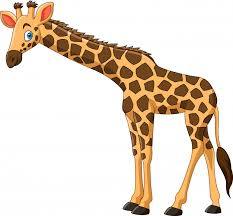
\includegraphics{images/giraffe.jpg}
	\caption{Giraffe}
	\label{fig:giraffe}
\end{figure}


\chapter{Dummy text}
\lipsum[2-3]


% Changes numbering of chapters to alphabetic form
\appendix
\chapter{Appendix}
\lipsum[2-3]



% Havard Style
\bibliographystyle{unsrtnat}
%\bibliographystyle{agsm}  % Incompatible with memoir since it uses \bf, which is deprecated.
\bibliography{references}


\end{document}